\section{Tests und Versuche}

\subsection{Mechanik}

Die Hauptaufmerksamkeit zu Beginn gilt dem Prozess des Schiessens/ Befördern 
der Bälle. Aus diesem Grund wird entschieden, einen Versuchsaufbau zu 
konstruieren, um diese Funktion auf ihre Zuverlässigkeit und Genauigkeit zu 
testen. Als erstens wird ein Aufbau hergestellt, welcher die Bälle mit Hilfe 
eines Rades beschleunigt. \\
%
Die Konstruktion besteht hauptsächlich aus Holz, das es dadurch relativ 
einfach ist Anpassungen vorzunehmen. Die Lagerung der Welle mit welcher das 
Rad aus dem Modellbau dreht, wird mit zwei im Holz eingepressten Kugellagern 
realisiert. Da die berechnete Drehzahl des Rades zwischen 700 U/min bis 900 
U/min liegt, muss ein passender Motor gefunden werden. Motoren in diesem 
Drehzahlbereich sind jedoch sehr rar. Aus diesem Grunde wird auf einen Motor 
welcher bei RC-Modellautos eingesetzt wird zurückgegriffen. Dieser hat jedoch 
eine Drehzahl von über 20'000 U/min und muss deshalb stark untersetzt werden, 
um die gewünschte Raddrehzahl zu erhalten. Die Untersetzung wird mit zwei 
Riemenscheiben und einem O-Ring gelöst. Dadurch wird eine Untersetzung von 
ca. 1:30 erreicht damit der Ball die richtige Abschussgeschwindigkeit erhält. 
Da dieser Motor leider einen relativ hohen Drehzahl Einbruch hat sobald ein 
Ball geschossen wird, muss nach einer Alternative gesucht werden. Der 
zweite Motor, mit welchem getestet wird, stammt aus dem Flugzeugmodellbau und 
ist ein Brushless Innenläufer Motor mit Getriebe. Mit diesem können die 
Bälle in sehr kurzen Abständen mit nahezu gleich bleibender Drehzahl geschossen 
werden. Der Abschusswinkel bei diesen Versuchen wird experimentell ermittelt 
und mit ca. 50$^\circ$ als optimal festgelegt. \\
%
Anschliessend wird ein Mechanismus gesucht mit welchem die Bälle 
gleichmässig zum Beschleunigungsrad geführt werden können, damit die Wurfweite 
nicht beeinflusst wird. Die Idee ist es, mit einem umschlingenden Band die 
Bälle nacheinander zuzuführen. Beim Versuch wird als Band eine 0.1 mm dicke 
Präzisionsstahlfolie verwendet. Diese zeichnet sich durch eine hohe Stabilität, 
Aufrollbarkeit und ein geringes Gewicht aus. Beim Test ist das Band auf der 
einen Seite befestigt, umschlingt alle Tennisbälle und wird kurz vor dem Rad 
durch einen Schlitz im Holz nach draussen geführt. Leider kann bis heute 
diese Technik nur manuell getestet werden, was so viel bedeutet wie, das Band 
wird von Hand beim Test hinausgezogen. \\
%
Den Test des Drehmechanismus kann leider noch nicht durchgeführt werden, da 
einzelne Komponenten noch fehlen und dadurch diese noch nicht kombiniert 
werden können um zu testen.

\subsection{Ultraschallsensor HC-SR04}
Diese Messung wird gemeinsam mit Gruppe 39 durchgeführt. \\
Ein sehr verbreitetes Modul für die Distanzmessung mittels Ultraschall ist 
das Modul HC-SR04. Mit diesem werden Messungen durchgeführt um festzustellen, 
ob es geeignet ist, einen Eimer zu detektieren. 

\subsubsection{Messmittel}
\begin{zebratabular}{lll}
    \rowcolor{gray} Gerät &
        Typ &
        Nummer \\
    Speisegerät &
        Hameg ... &
        SN ... \\
    Oszilloskop &
        Agilent &
        SN ... \\
    Pulsgenerator &
        Hameg &
        SN ... \\
    Mainframe &
        Hameg 800? &
        SN ... \\
\end{zebratabular}

\subsubsection{Ansteuerung}
\begin{zebratabular}{ll}
    \rowcolor{gray} Pin & Beschreibung \\
    VCC     & +5V DC \\
    Trig    & Trigger-Eingang (Startsignal) \\
    Echo    & Echo-Feedback \\
    GND     & MAsse (0V) \\
\end{zebratabular}

\subsubsection{Testeimer}
Als Testeimer wird der Abfalleimer aus dem Raum C200 verwendet. \\
\begin{zebratabular}{ll}
    \rowcolor{gray} Eigenschaft & Wert \\
    Durchmesser oben    & 38 cm \\
    Durchmesser unten   & 33 cm \\
    Höhe                & 48 cm \\
    Farbe               & schwarz (matt) \\
    Material            & Kunststoff () \\
    Hersteller          & Helit \\
    Typ                 & 61062 \\
\end{zebratabular}

\subsubsection{Messung Messgenauigkeit}
Die folgenden Werte sind statistisch aus mindestens 1000 Einzelmessugen 
ermittelt. \\
\begin{zebratabular}{lll}
    \rowcolor{gray} Abstand [cm] & Impuls mean [ms] & Std. Dev. [$\mu$s] \\
    50  & 2.987 & 2.4 \\
    60  & 3.503 & 2.4 \\
    70  & 4.060 & 10 \\
    80  & 4.766 & 24 \\
    90  & 5.230 & 10 \\
    100 & 5.807 & 11 \\
    110 & 6.413 & 13 \\
    120 & 7.040 & 16 \\
    130 & 7.722 & 22 \\
    140 & 8.229 & 16 \\
    150 & 8.854 & 15 \\
    160 & 9.500 & 43 \\
    170 & 10.06 & 22 \\
    180 & n.a.  & n.a. \\
\end{zebratabular} \\
Anschliessend wird eine weitere Messung durchgeführt. Dabei wird eine 
Holzplatte mit einem Abstand von 180 cm verwendet. Als Platte dient ein Tablar 
aus dem Raum B332c. Der Median beträgt 10.45 ms bei einer Standardabweichung 
von von 9.7 $\mu$s. \\
$\to$ Deutlich besseres Signal auf flachen Gegenständen als auf Runden. 

\subsubsection{Messung seitliche Empfindlichkeit}
Um die seitliche Empfindlichkeit zu testen, wird der Eimer unter einem 
bestimmten Winkel vor dem Sensor aufgestellt. Der Abstand wird dabei 
so eingestellt, dass der Sensor den Eimer gerade noch erkennt. Die erzielte
Distanz wird gemessen. \\
\begin{zebratabular}{ll}
    Winkel [$^\circ$] & Messbereich [cm] \\
    0   & 180 \\
    5   & 123 \\
    10  & 120 \\
    15  & 119 \\
    20  & 113 \\
    25  & 106 \\
    30  & 104 \\
    35  & 77  \\
    40  & 0   \\
\end{zebratabular} \\
Zwischen 25$^\circ$ und 30$^\circ$ hat der Sensor in einem Abstand von 75 bis 
90 cm einen blinden Bereich, in welchem der Eimer nicht erkannt wird. 

\subsubsection{Fazit}
Der Sensor ist nicht geeignet, um den Eimer zu finden, da der Sensor über 
einen zu breiten und zu ungenau definierten Winkel empfindlich ist. Der 
HC-SR04 wird somit nicht weiter als Sensor zur Detektion des Eimers 
weiterverfolgt. 

\subsection{Informatik}

\subsubsection{Versuchsbeschreibung}
Im Folgenden wird der Test von OpenCV in Java beschrieben. Es soll mittels des frei erhältlichen Frameworks OpenCV die Korbfindung ausgeführt werden.

\subsubsection{Vorbereitung}
Zu Testzwecken werden verschiedene Fotos von einem schwarzen Korb angefertigt. Es gibt zwei verschiedene Hintergrundszenarien. Bei jedem Hintergrund wird der Korb an 3 verschiedenen Stellen platziert.

Beispielbilder (jeweils eins bei jedem Hintergrund):

\begin{figure}[h!]
	\centering
	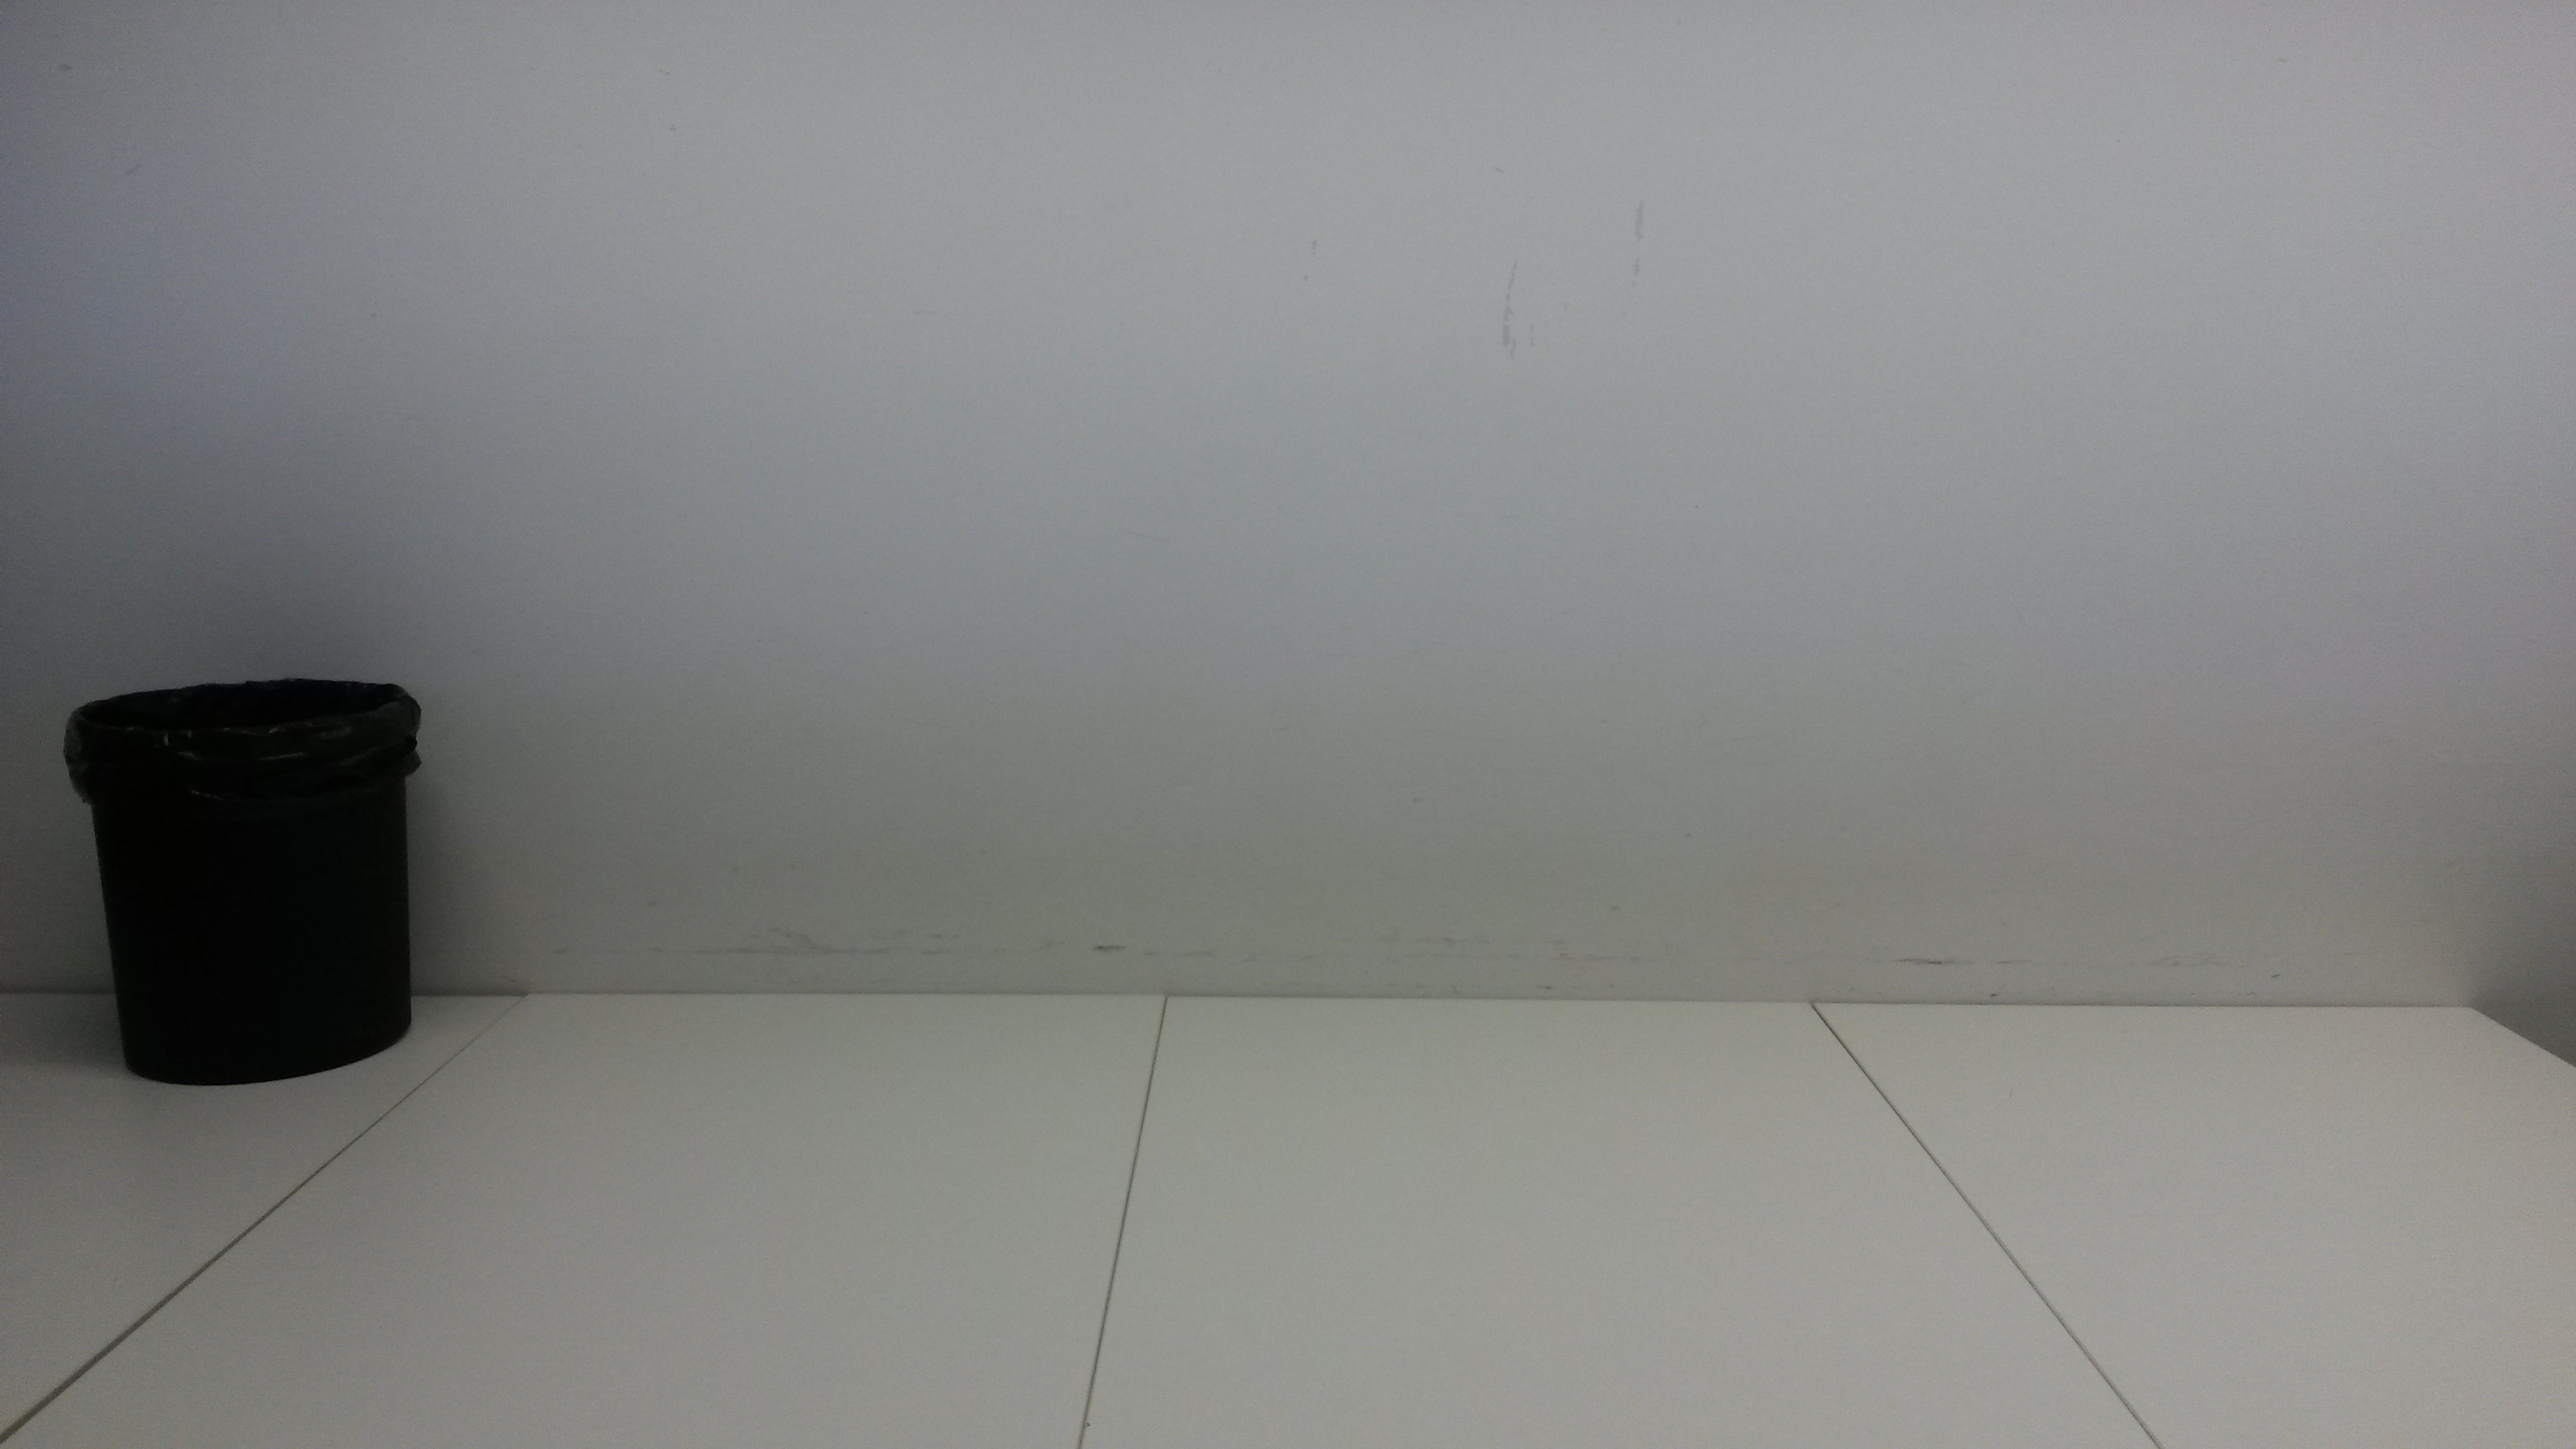
\includegraphics[width=0.5\textwidth]{fig/korb4.jpg}
	\caption{Hintergrund einfarbig}
	\label{fig:Korb_HEinfarbig}
\end{figure}

\begin{figure}[h!]
	\centering
	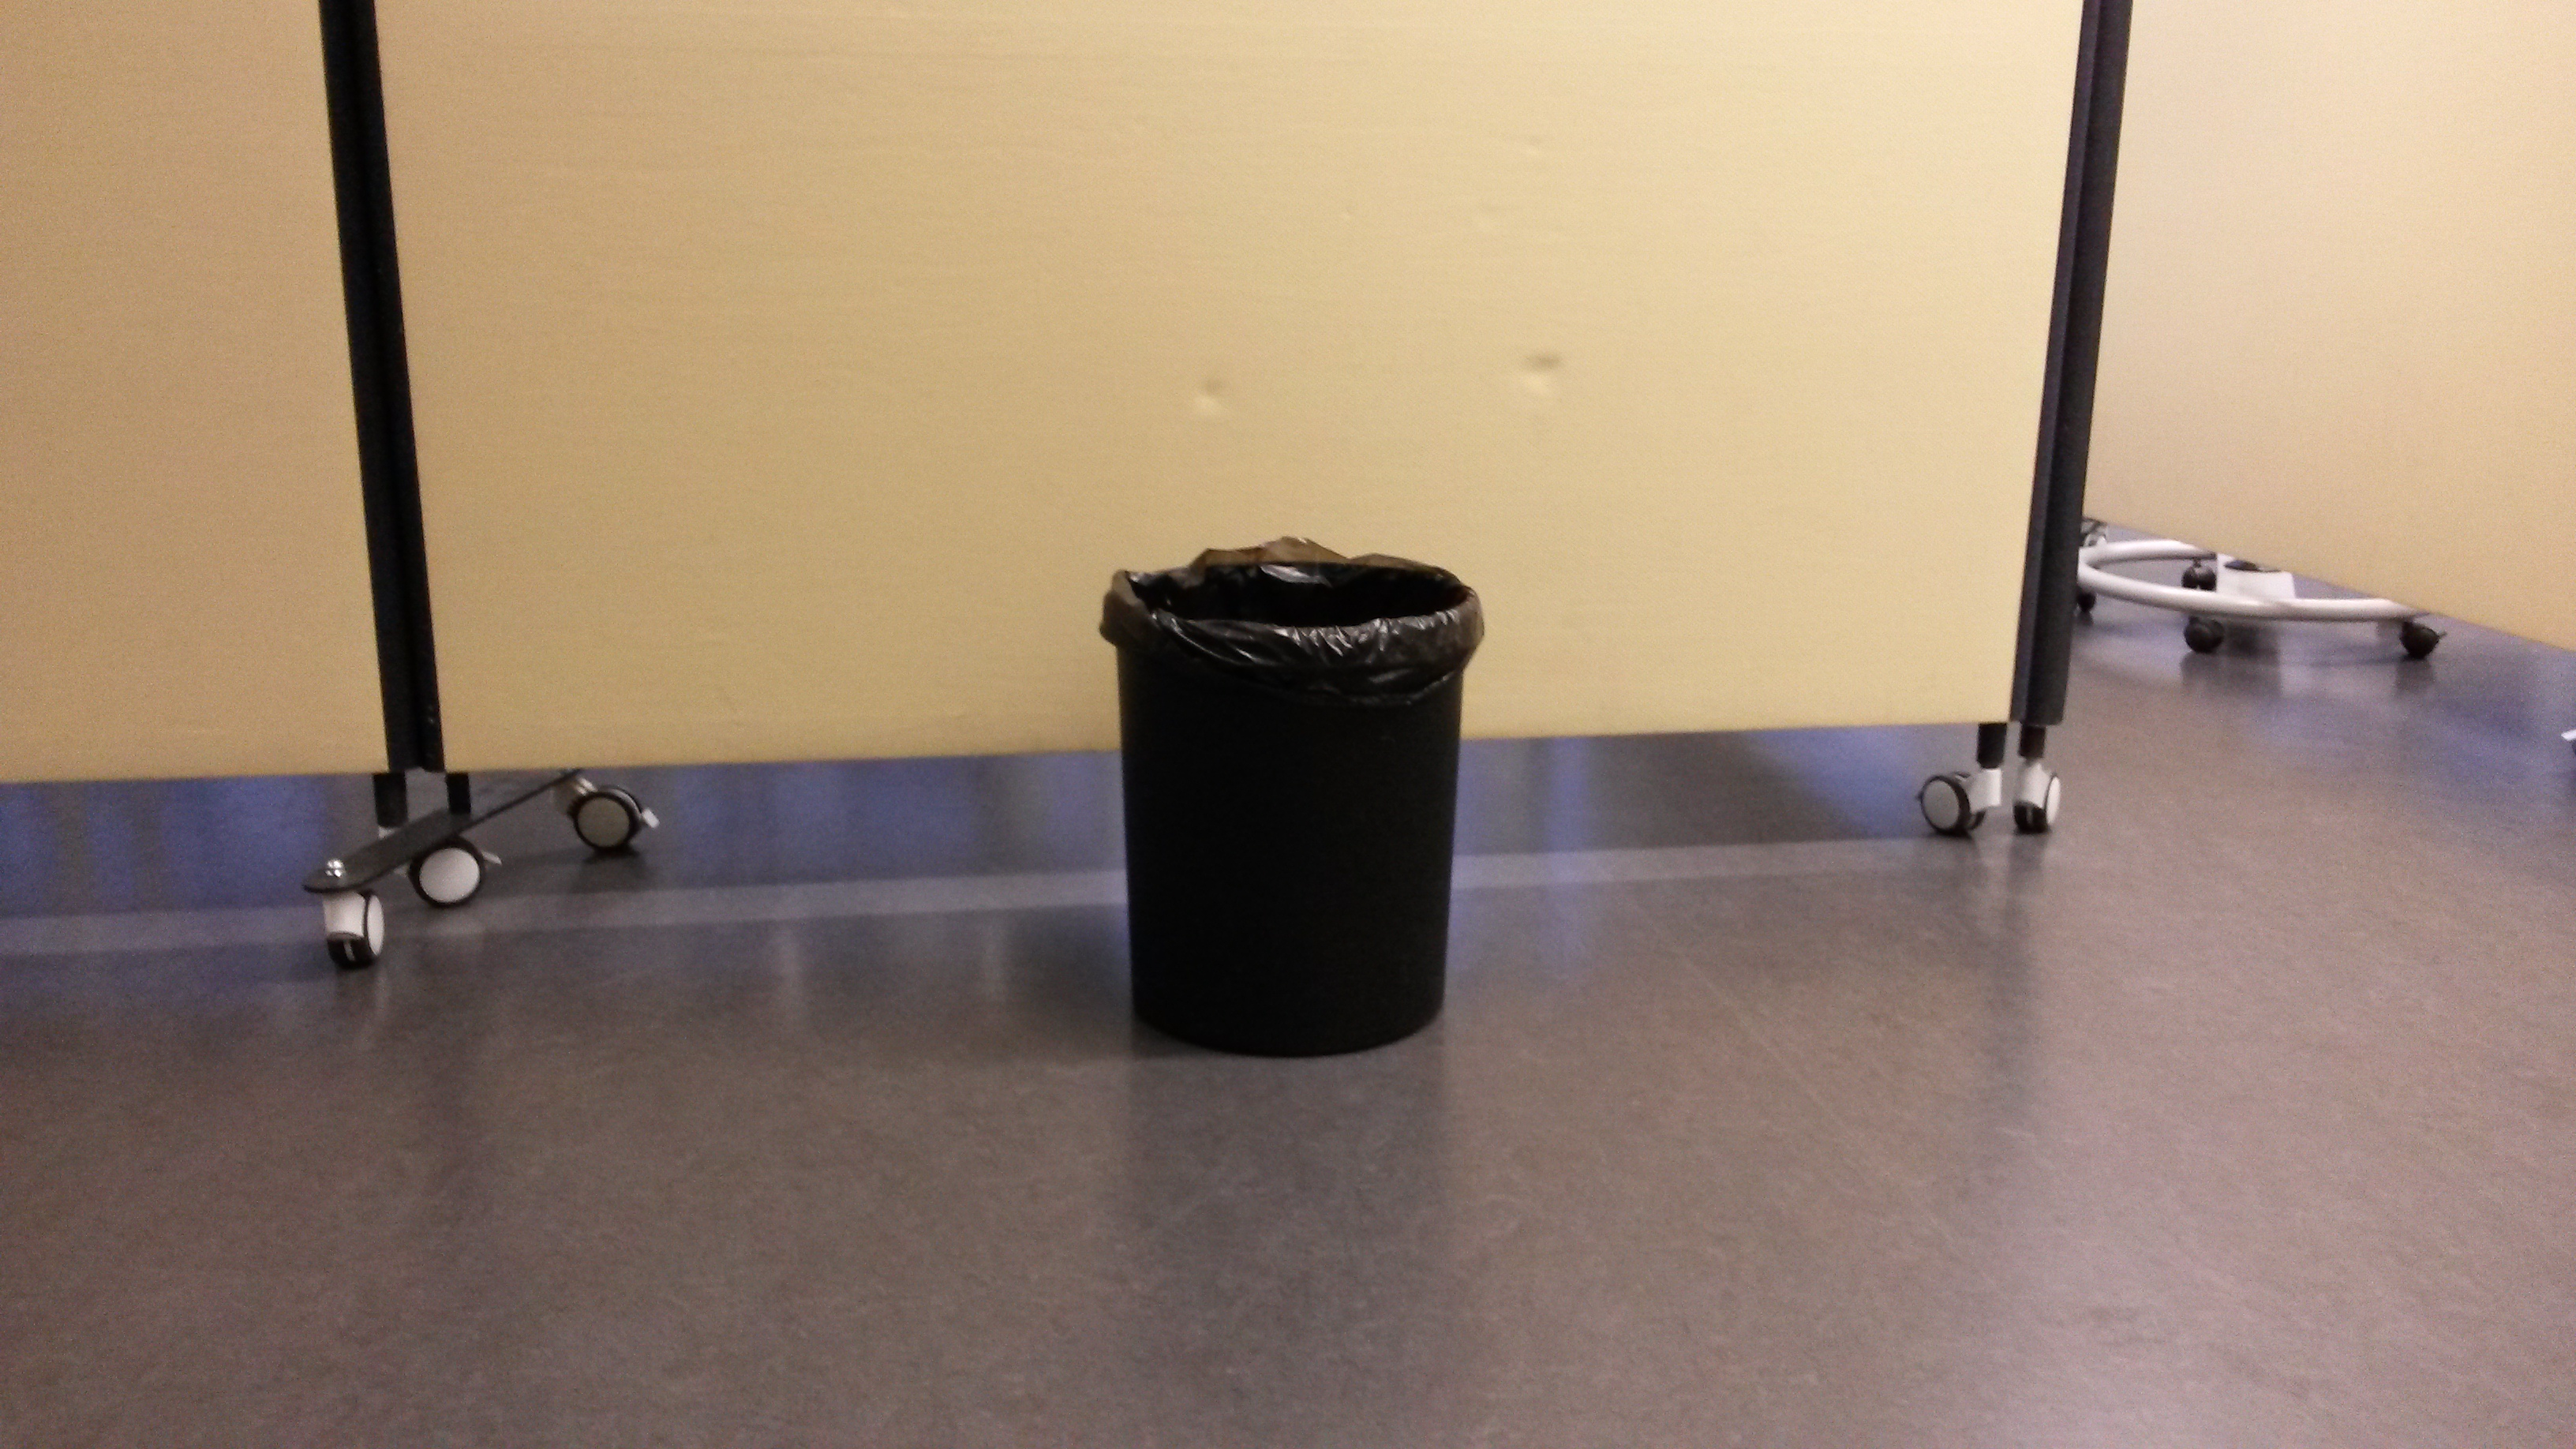
\includegraphics[width=0.5\textwidth]{fig/korb1.jpg}
	\caption{Hintergrund enthält schwarz}
	\label{fig:Korb_HSchwarz}
\end{figure}

Abbildung \ref{fig:Korb_HSchwarz} zeigt einen Hintergrund bei dem zusätzlich noch schwarze Farbe vorkommt. Dies erhöht den Schwierigkeitsgrad  den Korb zu erkennen. Da der Suchvorgang falsche Informationen verwerten kann. Bei Abbildung \ref{fig:Korb_HEinfarbig} ist der Hintergrund möglichst einfarbig gehalten um ein gegensätzliches Szenario zu Abbildung \ref{fig:Korb_HSchwarz} zu erhalten.

\subsubsection{Erkennung}
Im folgenden Bereich wird beschrieben wie das Vorgehen um den Korb zu erkennen gewählt wurde und einige Ergebnisse präsentiert.\\
%
Als erstes wird eines der Beispielbilder geladen.\\
%
Es folgen folgende Schritte:\\
%
\begin{itemize}
	\item Das Bild wird geladen und in ein HSV-Bild umgewandelt
	\begin{itemize}
		\item HSV steht für einen Farbwertebereich der mit Hughe, Saturation, Value beschrieben wird.
		\item Im Folgenden ein Bild des HSV-Farbbereichs:\\
		\begin{figure}[h!]
			\centering
			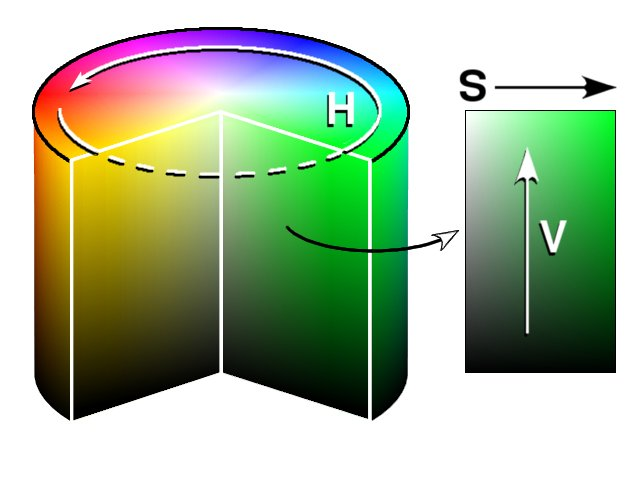
\includegraphics[width=0.5\textwidth]{fig/HSV_cylinder.jpg}
			\caption{HSV-Farbspektrum}
			\label{fig:HSV-Farbspektrum}
		\end{figure}
	\end{itemize}
	\item Es folgt eine HSV-Filterung. Dafür sind beim erstellten Programm 3 Slider angebracht. Um mit den Werten zu experimentieren und die optimalen Ergebnisse zu erzielen bei erzeugen eines Schwarz-Weiss Bildes
	\begin{itemize}
		\item Die 2 Slider für Hue und Saturation sind auf den Minimumwert 0 und Maximalwert 256 Eingestellt. Dieses können so belassen werden
		\item Der 3. Slider steht für den Value. Mit welchem die Dunklen werte gefiltert werden. Hier wird mit einer Grundeinstellung von Minimum 0 und Maximal 15 gearbeitet.
		\begin{itemize}
			\item Zum Experimentieren kann der Slider verschoben werden und der Filter erneut angewendet werden.
		\end{itemize}
	\end{itemize}
	\item Nach der Filterung ist das Bild noch von „Farb-Rauschen“ erfüllt. Dieses Rauschen wird mit dem „Eroden“ herausgefiltert.
	\begin{itemize}
		\item Für das erodieren wird mit 5*5 Pixel grossem Filter gearbeitet. Alles was diesem Wert entspricht wird von Weiss in Schwarz umgewandelt.
		\item So werden kleine ungewollte weisse Pixel aus dem Bild entfernt.
		\item Dieser Vorgang wird 2 Mal auf das Bild angewendet.
	\end{itemize}
	\item Nach dem Erodieren muss noch ein „Dilate“ ausgeführt werden.
	\begin{itemize}
		\item Damit werden ungewolltes entfernen wieder Rückgängig gemacht indem Pixelflächen wieder vergrössert werden.
		\item Hier wird mit einem Wert von 15*15 Pixeln gearbeitet.
		\item Das „Dilate“-Elements wird 2 Mal auf das Bild angewendet.
	\end{itemize}
	\item Nach diesen Massnahmen sollte nur noch der Korb als weisse Fläche auf dem Bild zu sehen sein und der Rest ist schwarz.
\end{itemize}

Ergebniss für die Abbildung \ref{fig:Korb_HEinfarbig} nach dem Anwenden der Filter sieht folgendermassen aus:

\begin{figure}[h!]
	\centering
	
\includegraphics[width=0.7\textwidth]{fig/Korberkennung1.png}
	\caption{Links nach Erode und Dilate - Rechts nur mit HSV Filterung}
	\label{fig:Korb_Erkennung}
\end{figure}

\subsubsection{Testprogramm}
Anbei sieht man ein Screenshot des Testprogramms:
\begin{figure}[h!]
	\centering
	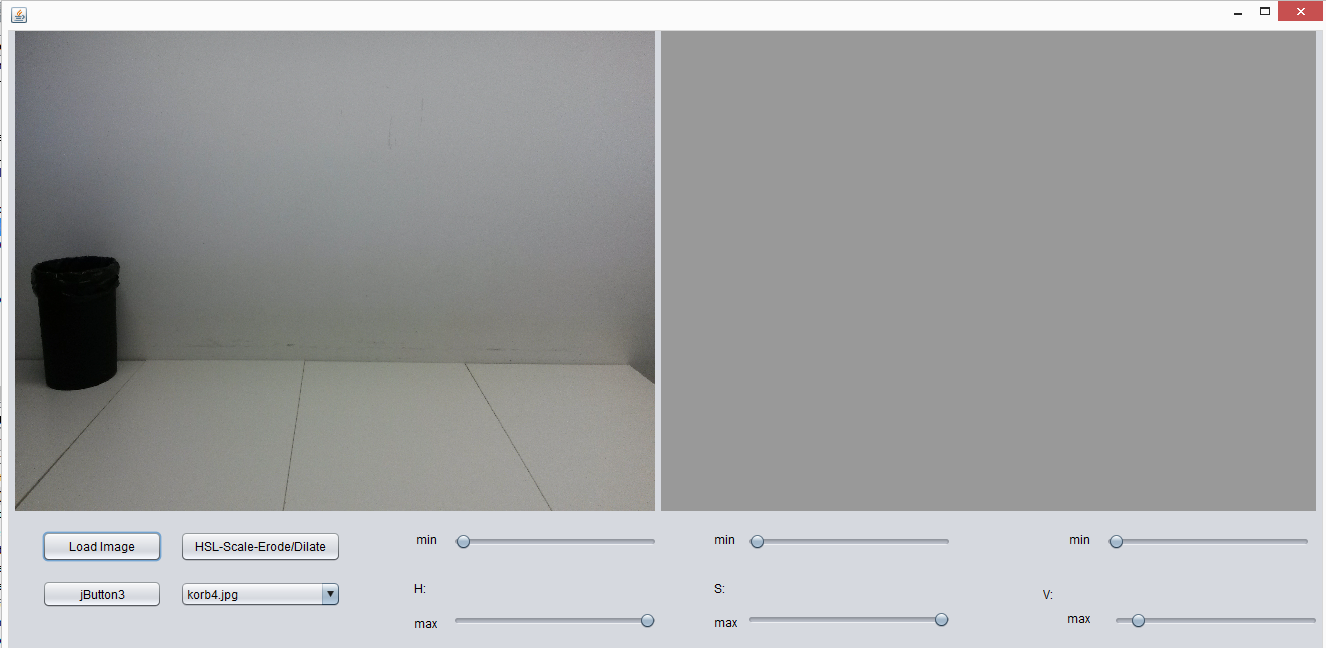
\includegraphics[width=0.7\textwidth]{fig/Testprogramm.png}
	\caption{Screenshot Testprogramm}
	\label{fig:Korb_Testprogramm}
\end{figure}

Abbildung \ref{fig:Korb_Testprogramm} zeigt die Einstellungsmöglichkeiten des Testprogramms. Es können mittels Slider die Werte für Hue, Saturation und Value angepasst werden. Nach einem Klick auf den Button wird der Filter mit den angegebenen HSV-Werten ausgeführt und in den zwei Bereichen dargestellt. Rechts nur der HSV-Filter und links mit dem erodieren und dem DIlate (wie in Abbildung 4 ersichtlich ist).
Über den Load Image Button können verschiedene Bilder geladen werden, welche in der Dropdownbox zur Verfügung stehen.
